\section{Homework Solutions (Yip)}
These are the solutions to Yip's Math/Stat 519 homework for the fall
semester of 2016.

Our main reference is \cite{ross}.

\subsection{Homework 1}
\subsubsection{Problems}
\begin{problem}[Ross, \S 1, \# 7]
  \hfill
  \begin{alphlist}
  \item In how many different ways can \(3\) boys and \(3\) girls sit in a
    row?
  \item In how many ways can \(3\) boys and \(3\) girls sit in a row if the
    boys and the girls are each to sit together?
  \item In how many ways if only the boys must sit together?
  \item In how many ways if no two people of the same sex are allowed to
    sit together?
  \end{alphlist}
\end{problem}
\begin{solution*}
\end{solution*}

\begin{problem}[Ross, \S 1, \# 11]
  In how many ways can \(3\) novels, \(2\) mathematics books, and \(1\)
  chemistry book be arranged on a bookshelf if
  \begin{alphlist}
  \item the books can be arranged in any order?
  \item the mathematics books must be together and the novels must be
    together?
  \item the novels must be together, but the other books can be arranged in
    any order?
  \end{alphlist}
\end{problem}
\begin{solution*}
\end{solution*}

\begin{problem}[Ross, \S 1, \# 19]
  From a group of \(8\) women and \(6\) men, a committee consisting of
  \(3\) men and \(3\) women is to be formed. How many different committees
  are possible if
  \begin{alphlist}
  \item \(2\) of the men refuse to serve together?
  \item \(2\) of the women refuse to serve together?
  \item \(1\) mand and \(1\) woman refuse to serve together?
  \end{alphlist}
\end{problem}
\begin{solution*}
\end{solution*}

\begin{problem}[Ross, \S 1, \# 21]
  Consider the grid of points show at the top of the next column (in the
  book; we draw it here using Asymptote).
  \[
    
\includegraphics{yip-1-1}
  \]
  Suppose that, starting at the point labeled \(A\), you can go one step up
  or one step to the right at each move. This procedure is continued until
  the point labeled \(B\) is reached. How many different paths from \(A\)
  to \(B\) are possible?

  \noindent\emph{Hint:} Note that to reach \(B\) from \(A\) you must take
  \(4\) steps to the right and \(3\) steps up.
\end{problem}
\begin{solution*}
\end{solution*}

\begin{problem}[Ross, \S 1, \# 22]
  In Problem \# 21, how many different paths are there from \(A\) to \(B\)
  that go through the point circled in the following lattice?
  \[
    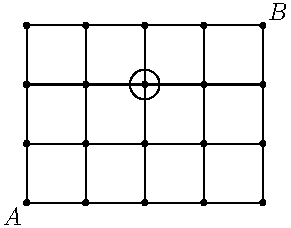
\includegraphics{yip-1-2}
  \]
\end{problem}
\begin{solution*}
\end{solution*}

\begin{problem}[Ross, \S 1, \# 33]
\end{problem}
\begin{solution*}
\end{solution*}

\subsubsection{Theoretical exercises}
\begin{problem}[Ross, \S 1, \# 5]
\end{problem}
\begin{solution*}
\end{solution*}

\begin{problem}[Ross, \S 1, \# 6]
\end{problem}
\begin{solution*}
\end{solution*}

\begin{problem}[Ross, \S 1, \# 8]
\end{problem}
\begin{solution*}
\end{solution*}

\begin{problem}[Ross, \S 1, \# 9]
\end{problem}
\begin{solution*}
\end{solution*}

\begin{problem}[Ross, \S 1, \# 12]
\end{problem}
\begin{solution*}
\end{solution*}

\begin{problem}[Ross, \S 1, \# 23]
\end{problem}
\begin{solution*}
\end{solution*}

\subsubsection{Problems}
\begin{problem}[Ross, \S 2, \# 25]
\end{problem}
\begin{solution*}
\end{solution*}

\begin{problem}[Ross, \S 2, \# 29]
\end{problem}
\begin{solution*}
\end{solution*}

\begin{problem}[Ross, \S 2, \# 35]
\end{problem}
\begin{solution*}
\end{solution*}

\begin{problem}[Ross, \S 2, \# 44]
\end{problem}
\begin{solution*}
\end{solution*}

\begin{problem}[Ross, \S 2, \# 49]
\end{problem}
\begin{solution*}
\end{solution*}

\subsubsection{Theoretical exercises}
\begin{problem}[Ross, \S 2, \# 5]
\end{problem}
\begin{solution*}
\end{solution*}

\begin{problem}[Ross, \S 2, \# 14]
\end{problem}
\begin{solution*}
\end{solution*}

\begin{problem}[Ross, \S 2, \# 19]
\end{problem}
\begin{solution*}
\end{solution*}

%%% Local Variables:
%%% mode: latex
%%% TeX-master: "../MA519-HW-ALL"
%%% End:
